% Charles McEachern

% Fall 2015

% This is a template for writing a note to Bob in TeX. 

\documentclass{article}

% =============================================================================
% ==================================== Package List Copied from Thesis Template
% =============================================================================

\usepackage{epsfig} % Allows the inclusion of eps files
\usepackage{epic} % Enhanced picture mode
\usepackage{eepic} % Extensions for epic
\usepackage{units} % SI unit typesetting
\usepackage{url} % URL handling
\usepackage{longtable} % Tables that continue onto multiple pages
\usepackage{mathrsfs} % Support for \mathscr script
\usepackage{multirow} % Span rows in tables
\usepackage{bigstrut} % Space struts in tables up and down
\usepackage{amssymb} % AMS math symbols and helpers
\usepackage{graphicx} % Enhanced graphics support
\usepackage{setspace} % Adjust spacing in captions, single by default
\usepackage{xspace} % Automatically adjusting space after macros
\usepackage{amsmath} % \text, and other math formatting options
\usepackage{siunitx} % \num{} formatting and SI unit formatting
\usepackage{booktabs} % Enhanced tables with \toprule, etc.
\usepackage{hyperref} % Add clickable links to other parts of the document
\usepackage[noabbrev]{cleveref} % Automatically determine \cref type

% Configure the siunitx package
\sisetup{
    group-separator = {,}, % Use , to separate groups of digits, like 12,345
    list-final-separator = {, and } % Always use the serial comma in \SIlist
}

\usepackage{parskip} % http://ctan.org/pkg/parskip

\usepackage{float} % Sometimes you want to tell LaTeX to put an image RIGHT HERE. 

% Configure the cleveref package
\newcommand{\creflastconjunction}{, and } % Always use the serial comma

\linespread{1.3}

% =============================================================================
% ============================================= Paper Spacing from Thesis Class
% =============================================================================

\setlength{\paperheight}{11.0in}
\setlength{\paperwidth}{8.5in}

%\setlength{\oddsidemargin}{1.937cm}  % default -> 2.0 cm odd side
%\setlength{\oddsidemargin}{0.55in} % final version to grad school
\setlength{\oddsidemargin}{0.55in}
\setlength{\evensidemargin}{0.1in} % default -> 3.4 cm even side
%\setlength{\evensidemargin}{0.1in} % default -> 3.4 cm even side

%\setlength{\topmargin}{0.75in}
\setlength{\topmargin}{0.25in}
%\setlength{\headheight}{0.0in}
\setlength{\headheight}{0.4in}
\setlength{\headsep}{0.1in}

\setlength{\marginparsep}{0in}
\setlength{\marginparwidth}{0in}

\setlength{\textwidth}{5.75in}
%\setlength{\textheight}{8.25in}
\setlength{\textheight}{7.85in}

\setlength{\footskip}{0.4in}

% =============================================================================
% ================================================================= Definitions
% =============================================================================

\newcommand{\Alfven}{Alfv\'en\xspace}

\newcommand{\Ampere}{Amp\`ere\xspace}

% =============================================================================
% ======================================================== Document Starts Here
% =============================================================================

\begin{document}

\section{29 January 2016}

Note that plots are PDF images. You can zoom in on them. 

\begin{figure}[H]
  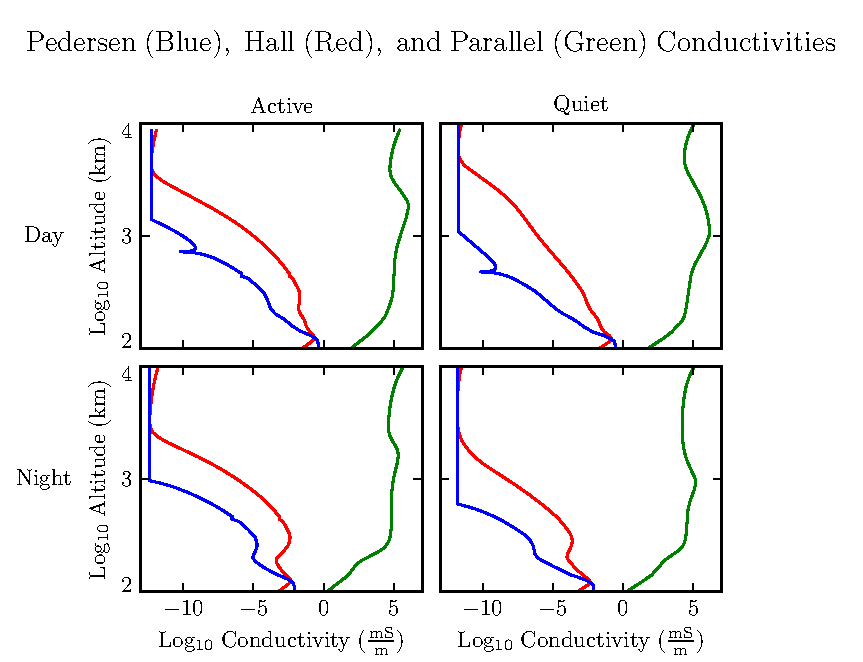
\includegraphics{sigma.pdf}
  \caption{These profiles come from Kelley's 1989 book. They have a significant effect on the behavior of \Alfven waves in the inner magnetosphere. To eyeball these effects, the following figures are plotted four-across, even though that cramps the axes.}
  \label{fig_sigma}
\end{figure}

\begin{figure}[H]
  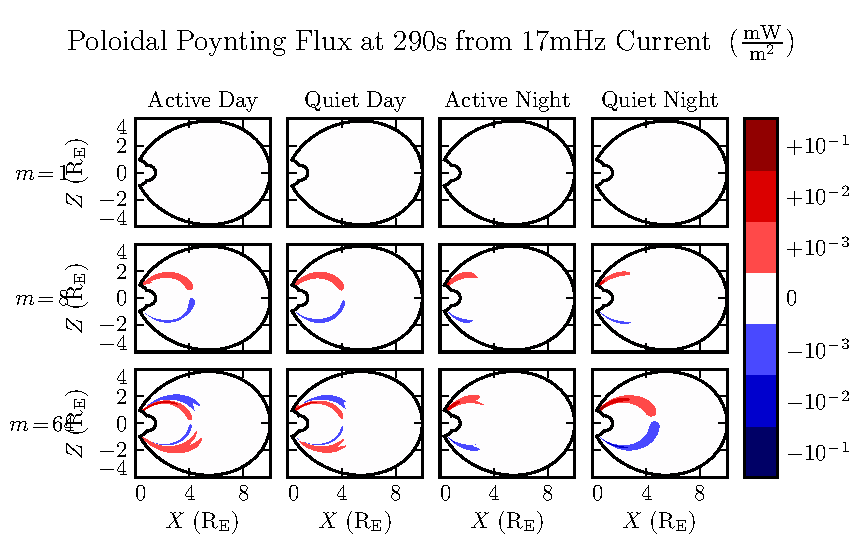
\includegraphics{SP.pdf}
  \caption{We drive with a poloidal electric field, which simulates perturbations in the azimuthal current. The strength of the response is affected by both the azimuthal modenumber and the ionospheric profile. That is, simply driving with a poloidal field does not guarantee a poloidal standing wave.}
  \label{fig_SP}
\end{figure}

\begin{figure}[H]
  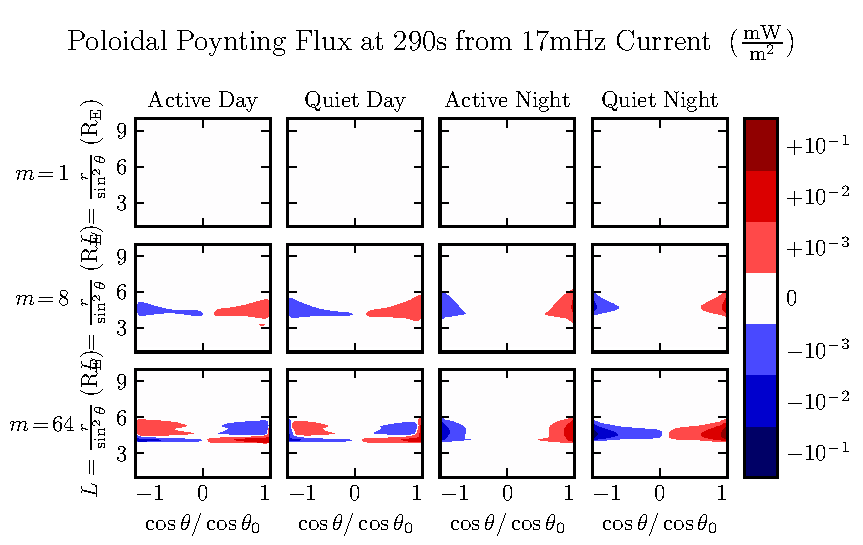
\includegraphics{SP_unwrapped.pdf}
  \caption{This is perhaps clearer when the dipole axes are unwrapped Here, each L shell is a horizontal line, and the horizontal axis has been renormalized to exaggerate the ionosphere. }
  \label{fig_SP_unwrapped}
\end{figure}

\begin{figure}[H]
  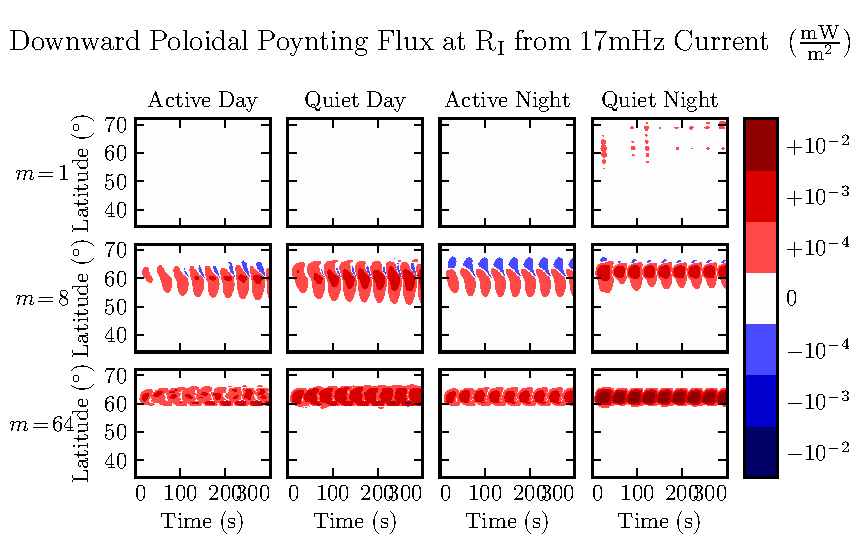
\includegraphics{SP_RI.pdf}
  \caption{Looking at the poloidal Poynting flux at the ionospheric boundary, it's again clear that both modenumber and conductivity play a role in field line resonance. At low $m$, energy decays from the poloidal mode to the toroidal mode before even reaching the ionospheric boundary. At high $m$, the poloidal Poynting flux is increased by orders of magnitude. When the conductivity is low, that energy is dissipated through Joule heating, but some upward Poynting flux is visible in the high-conductivity profiles.}
  \label{fig_SP_RI}
\end{figure}

\begin{figure}
  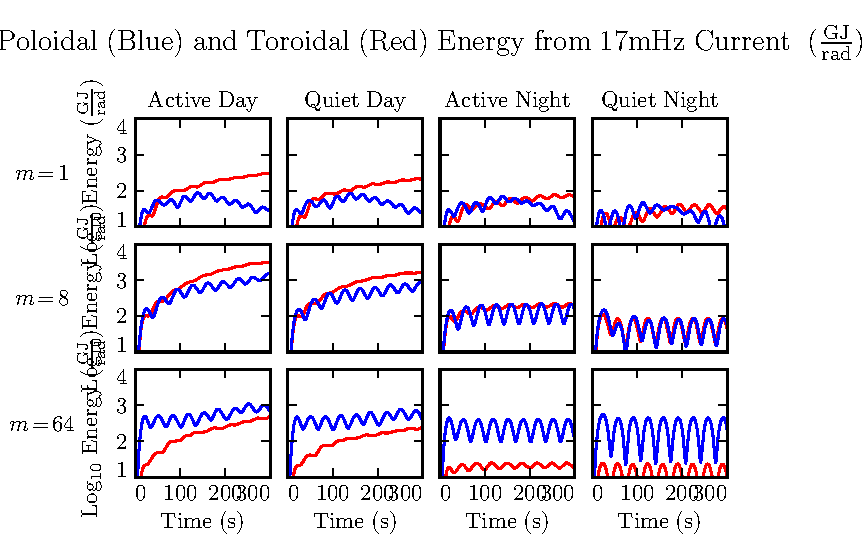
\includegraphics{UP_UT.pdf}
  \caption{This can be compared to Mann's results from 1995. Using a simple wave-in-a-box model, he found that the poloidal mode rotates to the toroidal mode in time proportional to $m$. Certainly, a stabler poloidal mode (and a slower-growing toroidal mode) are visible in high-$m$ simulations. But conductivity, which he neglected, is also an important consideration. On the night side, high $m$ gives a weaker toroidal mode, implying a slower rotation... but both curves look like damped-driven oscillators, not resonant ones.\hspace{\textwidth}This ties in nicely to a point made by Dai in his 2015 paper: it's not known why Pc4 pulsations are overwhelmingly observed on the dayside, when we would expect the driving mechanism (drift-resonant ions) to be broadly distributed in MLT. The answer may be that such waves are driven at at all MLT, but only observed where they're resonant. }
  \label{fig_UP_UT}
\end{figure}

\begin{figure}
  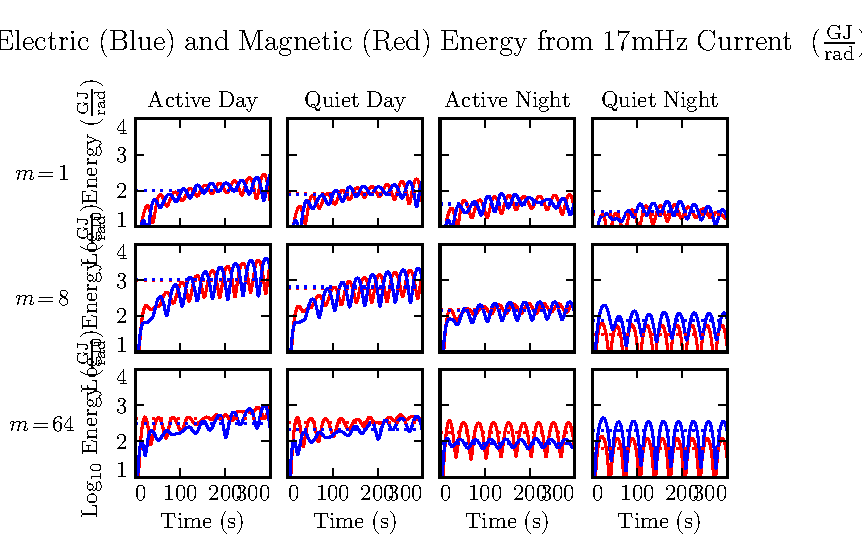
\includegraphics{UB_UE.pdf}
  \caption{Along the same line of reasoning, it's interesting to consider whether the modenumber or profile might affect the distribution of energy between the electric and magnetic fields. It seems that at low $m$, energy is distributed evenly between electric and magnetic fields, but that the distribution becomes lopsided as $m$ becomes large. When the conductivity is high, the magnetic fields are (on average) more energetic than the electric fields, and vice versa. }
  \label{fig_UB_UE}
\end{figure}

\begin{figure}
  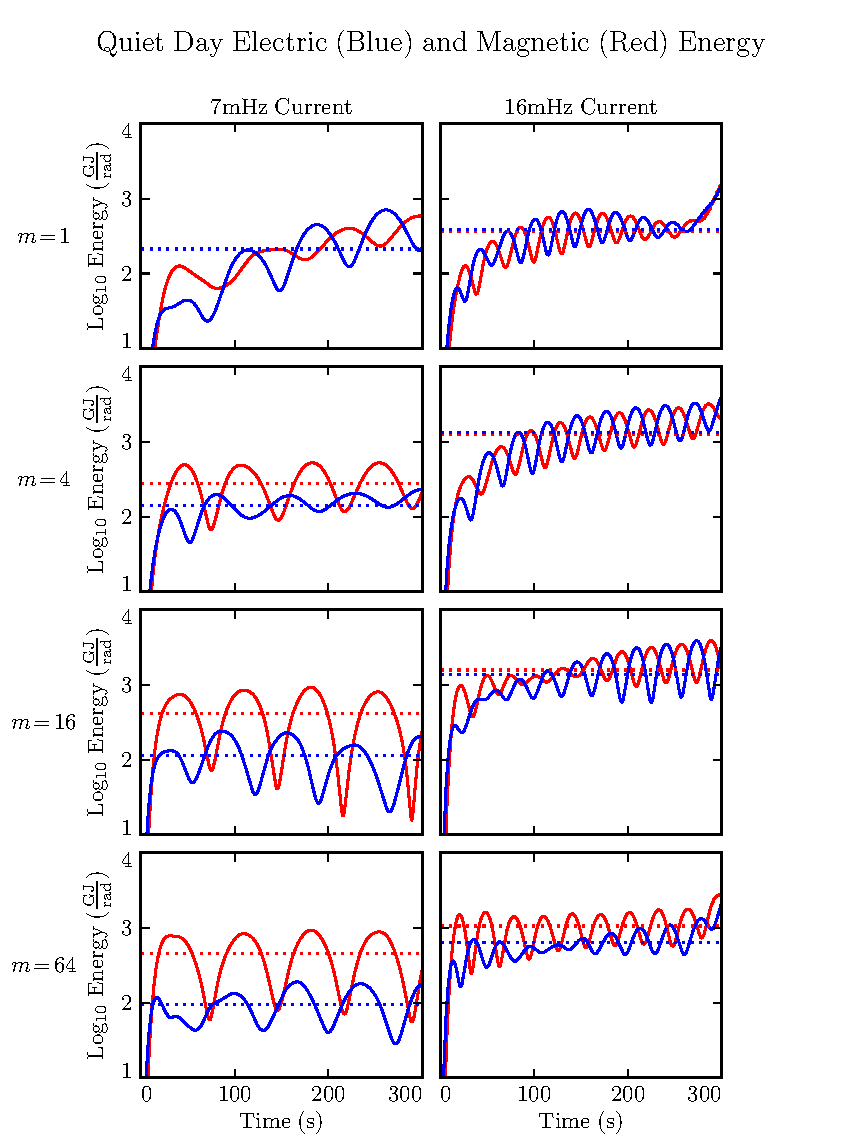
\includegraphics{UB_UE_slow.pdf}
  \caption{The lopsided energy distribution between electric and magnetic fields -- again, so far just based on a few runs -- seems to be most visible when the driving frequency is low. In the bottom-left plot, for example, the mean energy in the magnetic field is just over four times the mean energy in the electric field. }
  \label{fig_UB_UE_slow}
\end{figure}




\end{document}













